\section{Introduction}
\label{sec:intro}

There is a growing interest in applying conversational agents (i.e., chatbots) in the mental health domain~\cite{sabour2022chatbots}. Chatbots that can (i) conduct diagnosis conversations like a psychiatrist or (ii) simulate patients in the psychiatric diagnostic scenarios, have significant real-world applications\footnote{For the sake of clarity, we will refer to these two types of chatbots as the \textbf{``doctor chatbot''} and \textbf{``patient chatbot''} respectively in the subsequent sections.}. 
Doctor chatbots can be effective tools for mental disorder screening~\cite{pacheco2021Smart} in lieu of official medical diagnosis. Patient chatbots can serve as Standard Patients (SP) in medical education, making the learning process more efficient and cost-effective~\cite{Torous2021growing}.

However, there is still limited exploration in developing and evaluating these 
chatbots, primarily due to the difficulty in obtaining dialogue data because 
of the ethical and privacy concerns for mental health issues. 
% \KZ{you just said earlier that conversational agents are increasingly being used in mental health, but now you say limited exploration. Contradictory?} 
What's more, in outpatient scenarios, depressed patients often find it difficult 
to describe their ambiguous mental state objectively, 
and they may even be ashamed or afraid of disclosing their true 
conditions~\cite{Salaheddine2016Identify}. As a result, doctor chatbots should 
go beyond serving as interactive scales (e.g., PHQ-9) for mental disorder 
screening~\cite{Yue2023Beyond}. They need to possess various professional 
skills, including emotional support, to effectively complete the diagnosis task.
Additionally, patient chatbots should resemble real patients more closely, 
rather than precisely and robotically reporting their symptoms without 
any emotional fluctuations.

\begin{figure*}[th]
	\centering
	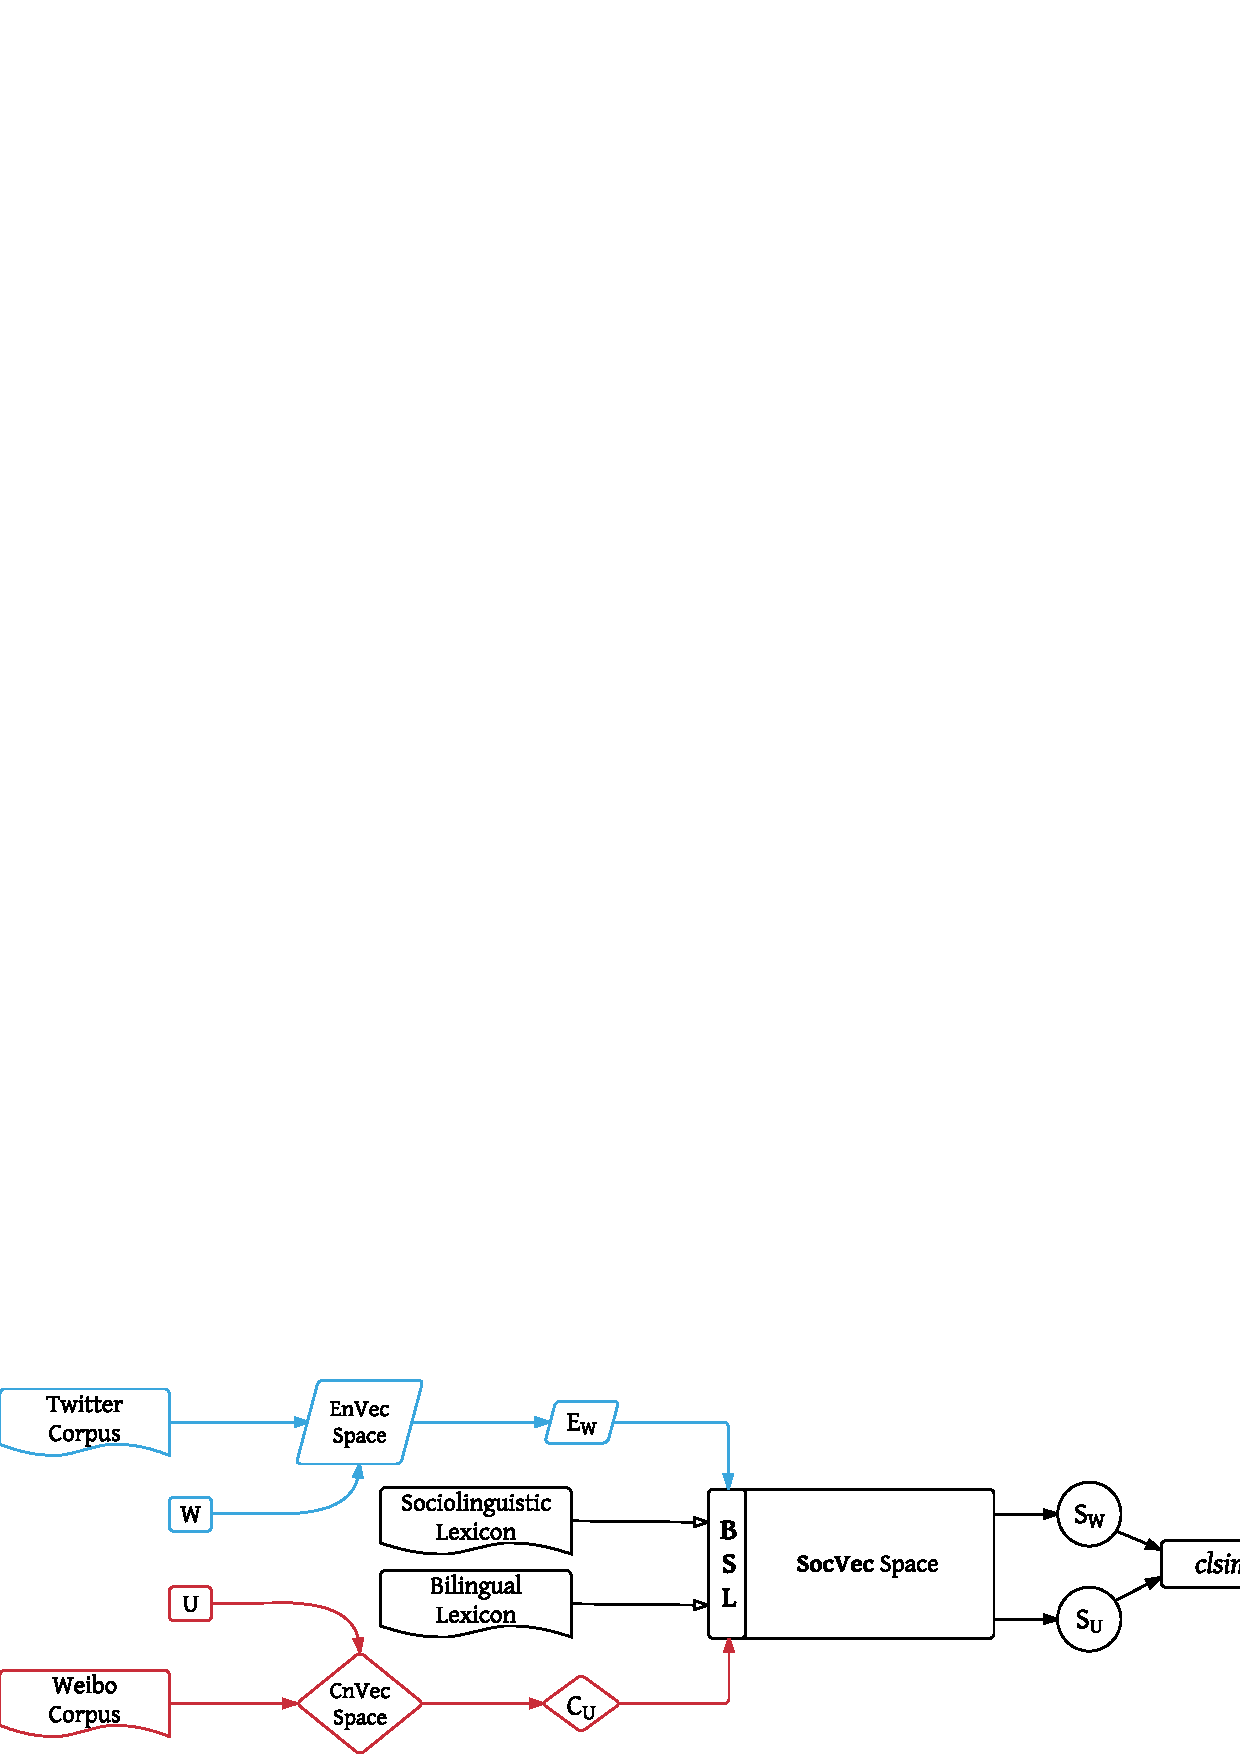
\includegraphics[width=0.8\linewidth]{Figures/overview.png}
	\caption{The overview of the expert-guided three-phase study.}
	\label{fig:pipeline}
\end{figure*}

% However, many existing frameworks~\cite{Medeiros2018UsingCF,Jaiswal2019Virtual} still rely on rule-based approaches (e.g., utilize the questions in self-rating scales), which often result in rigid conversations and cannot show sufficient empathy to patients. Alternatively, other deep learning methods \cite{yao-etal-2022-d4} require a significant amount of domain-specific data for training, which is often costly and difficult to obtain, especially in the mental health domain. 
% Furthermore, due to the diverse ways to express mental states verbally, neither rule-based nor data-based methods can comprehensively cover all possible cases, so the patient chatbots developed using these methods tend to be inflexible and lack diversity~\cite{Yao2020Toward}.

% \KZ{But how is simulating doctors and patient in diagnosis conversation more difficult than the therapeutic bots in Woebot and Wysa, and the like? In other words, why can't we use the techniques in Woebot and Wysa to simulate doctors and patients? I think the difference between diagnostic bots and therapeuric bots is that it's easier to verify quality of the doctor bot or patient bot: a good doctor bot must be able to acquire enough info efficiently from the patient so as to make a correct diagnosis; a good patient bot must resemble the real patient in doctors eyes. A good therapist however can't be easily qualified because all they are doing is to make the patient feel better, which is very subjective from the patient point of view.}  


Achieving these goals is quite difficult for conventional rule-based~\cite{Medeiros2018UsingCF,Jaiswal2019Virtual} or even data-driven~\cite{yao-etal-2022-d4, Fansi2022DDXPlus, Lin2021Graph} methods. This difficulty arises from the complexity of understanding varied human utterance in diagnosis conversations with a limited amount of pre-defined rules or training data. 
% \MY{Any reason why data-drive is not enough as well?} 
Fortunately, recent advancements in large language models (LLMs), such as ChatGPT\footnote{\url{https://chat.openai.com/}}, provide a new way to develop chatbots that can convincingly portray specific roles for its superior capability in understanding diverse natural language~\cite{Pan2023APE} and generating coherent conversations. Importantly, LLMs can achieve this with appropriate prompts rather than fine-tuning on extensive domain data.

% Equipped with comprehensive training data and knowledge, LLMs can generate diverse tones and symptom descriptions with appropriate prompts rather than fine-tuning on extensive domain data.\MY{what i meant is that why LLM can do it is not only because of its strength in generation but also understanding, these should be aligned with the challenges when using data-drive approaches}


% Achieving these goals is quite difficult for conventional rule-based~\cite{Medeiros2018UsingCF,Jaiswal2019Virtual} or even data-driven~\cite{yao-etal-2022-d4, Fansi2022DDXPlus, Lin2021Graph} methods, due to the difficulty of adequately covering complex cases of psychiatric diagnosis with a limited amount of pre-defined rules or training data. 
% % \MY{Any reason why data-drive is not enough as well?} 
% Fortunately, recent advancements in large language models (LLMs), such as ChatGPT\footnote{\url{https://chat.openai.com/}}, provide a new way to develop chatbots that can convincingly portray specific roles\MY{for its superior capability in understanding diversed natural language and generating coherant coversations, better add a ref}.  Equipped with comprehensive training data and knowledge, LLMs can generate diverse tones and symptom descriptions with appropriate prompts rather than fine-tuning on extensive domain data.\MY{what i meant is that why LLM can do it is not only because of its strength in generation but also understanding, these should be aligned with the challenges when using data-drive approaches}

% COMMENT: 前面所述,该chatbot的困难有两点:数据难采集和症状的模糊、主观。这里只讲清楚了ChatGPT能够解决数据采集的问题,那么它怎么来应对症状模糊主观的问题呢?此外还包括刚才上一段提到的,diagnosis chatbot需要提供情感支撑,patient simulator要仿真病人的情绪波动,要如何实现,这里是不是都应该简单描述一下?

Therefore, in this work, we aim to (i) respectively investigate the potential of ChatGPT in simulating \textit{psychiatrists} and depressed \textit{patients} in a clinical diagnosis scenario, 
as well as to (ii) build a comprehensive evaluation framework for these chatbots, answering the question about what constitutes a good psychiatrist chatbot and a truly patient-like chatbot.

To develop and evaluate a system that truly meets the the user's expectations, 
we follow a expert-guided design methodology. The study consists of three 
phases (See Figure~\ref{fig:pipeline}).
In \textbf{Phase 1}, as there lacks a formal description of the objectives for 
doctor and patient chatbots, we first collaborate with psychiatrists to 
identify them clearly. 
Based on these objectives, we conduct an experimental study 
(\textbf{Phase 2}) to design appropriate prompts for ChatGPT-based chatbots 
and establish an evaluation framework that incorporates both human evaluation 
and automatic evaluations aligned with the objectives from Phase 1. Importantly, the design of prompts and metrics was iterated based on human feedback, with each version improved with input from psychiatrists.
In \textbf{Phase 3}, we recruit real psychiatrists and depression patients to 
engage in diagnostic conversations with the 
simulated patient and doctor chatbots, respectively, and collect their 
ratings after conversation.
% We also conduct a comparison between the behavior of real and simulated psychiatrists based on the dialogue history, which yields some interesting findings. 

The main contributions of this work are:
\begin{itemize}
    \item We formalize the task of developing doctor and patient chatbots for depression diagnosis within an outpatient setting. In doing so, we propose specific \textit{objectives} for these chatbots that are up to near-clinical standards and establish an \textit{evaluation framework} that aligns with these objectives, with the help of practicing psychiatrists.
    \item We adopt an iterative prompt engineering approach, taking into account psychiatrists' feedback to refine the performance. By utilizing \textit{examples}, we enhance ChatGPT's understanding of professional practices. We further implement a \textit{reminder} mechanism to mitigate potential issues of forgetting when the desired behavior of chatbot being different from LLM's training purpose.
    % \MY{why is forgetting so common in our application, if it is a general phenomenon, we might want to change the reminder as patient behaviour being different from LLM's training purpose}
    \item We demonstrate the feasibility of utilizing ChatGPT-powered chatbots in mental health domain. Experiments show that ChatGPT-based doctor chatbot provides more accurate diagnostic results through more empathetic and efficient conversations with patients, comparing to the previous machine-learned chatbots.
    % \KZ{This is the first time you mention ``data-driven chatbot''. What exactly is it? Are you referring to CPT only?} 
    Moreover, the patient chatbot also exhibits emotional expression and 
resistance, which is similar to real patients. 
    % \item We suggest a data augmentation strategy that employs carefully evaluated doctor and patient chatbots to produce unlimited psychiatric outpatient dialogue data, effectively tackling the obstacle of obtaining data due to ethical concerns in mental health domain. We also provide the dataset containing dialogues between chatbots and real patients or psychiatrists from our evaluation experiments, which has been anonymized for privacy. 
    % \KZ{Ethical and privacy concerns?}
\end{itemize}




% Intuitively, relying on traditional evaluation metrics for dialogue systems (e.g., n-gram overlap, semantic textual similarity) to assess the performance of doctor and patient chatbots in mental health scenarios is inadequate, as there is no standardized answer for clinical conversations. 
% Moreover, what constitutes an exceptional psychiatrist chatbot or a realistic patient chatbot still remains unexplored. 

% Applications designed for mental health therapy or coaching in daily life, such as Woebot\footnote{\url{https://woebothealth.com}} and Wysa\footnote{\url{https://www.wysa.com}}, are gaining widespread attention for their ability to reduce users' negative emotions~\cite{Grove2021Codevelop} and promote a healthy lifestyle~\cite{Fadhil2019AssistiveCA}. Another notable application is chatbot-based symptom checkers~\cite{Yue2023Beyond}, which emulate human-like conversations while assessing users' symptoms, resembling interactive questionnaires.

